\documentclass[a4paper,10pt,twoside]{article}

\usepackage[top=1in, bottom=1in, left=1in, right=1in]{geometry}
\usepackage[utf8]{inputenc}
\usepackage[spanish,es-ucroman,es-noquoting]{babel}
\usepackage{setspace}
\usepackage{fancyhdr}
\usepackage{lastpage}
\usepackage{amsmath}
\usepackage{amsfonts}
\usepackage{verbatim}
\usepackage{graphicx}
\usepackage{float}
\usepackage{algorithmic}
\usepackage{tikz}
\usepackage{ gensymb }
\usetikzlibrary{calc}
\usetikzlibrary{decorations.pathreplacing}


% Evita que el documento se estire verticalmente para ocupar
% el espacio vacío en cada página.
\raggedbottom


%%%%%%%%%% Configuración de Fancyhdr - Inicio %%%%%%%%%%
\pagestyle{fancy}
\thispagestyle{fancy}
\lhead{RTP2, Organización del Computador II}
\renewcommand{\footrulewidth}{0.4pt}
\cfoot{\thepage /\pageref{LastPage}}

\fancypagestyle{caratula} {
   \fancyhf{}
   \cfoot{\thepage /\pageref{LastPage}}
   \renewcommand{\headrulewidth}{0pt}
   \renewcommand{\footrulewidth}{0pt}
}
%%%%%%%%%% Configuración de Fancyhdr - Fin %%%%%%%%%%


%%%%%%%%%% Configuración de Algorithmic - Inicio %%%%%%%%%%
% Entorno propio para customizar la presentación del pseudocódigo
\newenvironment{pseudocodigo}
    {\vspace{0.5em} \begin{algorithmic}}
    {\end{algorithmic} \vspace{0.5em}}

% Alinear comentarios a la derecha
\renewcommand{\algorithmiccomment}[1]{\hfill \{#1\}}
%%%%%%%%%% Configuración de Algorithmic - Fin %%%%%%%%%%


%%%%%%%%%% Macros de tikz - Inicio %%%%%%%%%%
% Uso: \registroCuatro{etiqueta}{x}{y}{a4}{a3}{a2}{a1}
\newcommand{\registroCuatro}[7]{
    \ifthenelse{\equal{#1}{}}{}{
        \draw (#2, {#3 + 0.5}) node[anchor=east]{#1};
    }

    \draw   (#2, #3) rectangle +(4, 1) +(2, 0.5) node{#4}
          ++(4, 0)   rectangle +(4, 1) +(2, 0.5) node{#5}
          ++(4, 0)   rectangle +(4, 1) +(2, 0.5) node{#6}
          ++(4, 0)   rectangle +(4, 1) +(2, 0.5) node{#7};          
}

% Uso: \registroOcho{etiqueta}{x}{y}{a8}{a7}{a6}...{a1}
\newcommand{\registroOcho}[9]{
    \def\etiqueta{#1}
    \def\x{#2}
    \def\y{#3}
    \def\aviii{#4}
    \def\avii{#5}
    \def\avi{#6}
    \def\av{#7}
    \def\aiv{#8}
    \def\aiii{#9}
    \registroOchoX    
}
\newcommand{\registroOchoX}[2]{ % Auxiliar - no usar directamente
    \def\aii{#1}
    \def\ai{#2}
    \ifthenelse{\equal{\etiqueta}{}}{}{
        \draw (\x, {\y + 0.5}) node[anchor=east]{\etiqueta};
    }
    \filldraw[fill=white]
        (\x, \y) rectangle +(2, 1) +(1, 0.5) node{\aviii}
        ++(2, 0) rectangle +(2, 1) +(1, 0.5) node{\avii}
        ++(2, 0) rectangle +(2, 1) +(1, 0.5) node{\avi}
        ++(2, 0) rectangle +(2, 1) +(1, 0.5) node{\av}
        ++(2, 0) rectangle +(2, 1) +(1, 0.5) node{\aiv}
        ++(2, 0) rectangle +(2, 1) +(1, 0.5) node{\aiii}
        ++(2, 0) rectangle +(2, 1) +(1, 0.5) node{\aii}
        ++(2, 0) rectangle +(2, 1) +(1, 0.5) node{\ai};
}


% Uso: \registroDieciseis{etiqueta}{x}{y}{a16}{a15}{a14}...{a1}
\newcommand{\registroDieciseis}[9]{
    \def\etiqueta{#1}
    \def\x{#2}
    \def\y{#3}
    \def\axvi{#4}
    \def\axv{#5}
    \def\axiv{#6}
    \def\axiii{#7}
    \def\axii{#8}
    \def\axi{#9}
    \registroDieciseisX
}
\newcommand{\registroDieciseisX}[9]{ % Auxiliar - no usar directamente
    \def\ax{#1}
    \def\aix{#2}
    \def\aviii{#3}
    \def\avii{#4}
    \def\avi{#5}
    \def\av{#6}
    \def\aiv{#7}
    \def\aiii{#8}
    \def\aii{#9}
    \registroDieciseisXX
}
\newcommand{\registroDieciseisXX}[1]{ % Auxiliar - no usar directamente
    \def\ai{#1}
    \ifthenelse{\equal{\etiqueta}{}}{}{
        \draw (\x, {\y + 0.5}) node[anchor=east]{\etiqueta};
    }
    \filldraw[fill=white]
        (\x, \y) rectangle +(1, 1) +(0.5, 0.5) node{\axvi}
        ++(1, 0) rectangle +(1, 1) +(0.5, 0.5) node{\axv}
        ++(1, 0) rectangle +(1, 1) +(0.5, 0.5) node{\axiv}
        ++(1, 0) rectangle +(1, 1) +(0.5, 0.5) node{\axiii}
        ++(1, 0) rectangle +(1, 1) +(0.5, 0.5) node{\axii}
        ++(1, 0) rectangle +(1, 1) +(0.5, 0.5) node{\axi}
        ++(1, 0) rectangle +(1, 1) +(0.5, 0.5) node{\ax}
        ++(1, 0) rectangle +(1, 1) +(0.5, 0.5) node{\aix}
        ++(1, 0) rectangle +(1, 1) +(0.5, 0.5) node{\aviii}
        ++(1, 0) rectangle +(1, 1) +(0.5, 0.5) node{\avii}
        ++(1, 0) rectangle +(1, 1) +(0.5, 0.5) node{\avi}
        ++(1, 0) rectangle +(1, 1) +(0.5, 0.5) node{\av}
        ++(1, 0) rectangle +(1, 1) +(0.5, 0.5) node{\aiv}
        ++(1, 0) rectangle +(1, 1) +(0.5, 0.5) node{\aiii}
        ++(1, 0) rectangle +(1, 1) +(0.5, 0.5) node{\aii}
        ++(1, 0) rectangle +(1, 1) +(0.5, 0.5) node{\ai};
}
%%%%%%%%%% Macros de tikz - Fin %%%%%%%%%%


%%%%%%%%%% Macros misceláneos - Inicio %%%%%%%%%%
\newcommand{\xmm}[1]{\texttt{XMM#1}}
\newcommand{\rax}{\texttt{RAX}}
\newcommand{\rbx}{\texttt{RBX}}
\newcommand{\rcx}{\texttt{RCX}}
\newcommand{\rdx}{\texttt{RDX}}
\newcommand{\rbp}{\texttt{RBP}}
\newcommand{\rsp}{\texttt{RSP}}
\newcommand{\reg}[1]{\texttt{R#1}}
\newcommand{\asm}[1]{\texttt{\uppercase{#1}}}
\newcommand{\INDSTATE}[1][1]{\STATE\hspace{#1\algorithmicindent}}
%%%%%%%%%% Macros misceláneos - Fin %%%%%%%%%%


\begin{document}


%%%%%%%%%%%%%%%%%%%%%%%%%%%%%%%%%%%%%%%%%%%%%%%%%%%%%%%%%%%%%%%%%%%%%%%%%%%%%%%
%% Carátula                                                                  %%
%%%%%%%%%%%%%%%%%%%%%%%%%%%%%%%%%%%%%%%%%%%%%%%%%%%%%%%%%%%%%%%%%%%%%%%%%%%%%%%


\thispagestyle{caratula}

\begin{center}


\includegraphics[height=2cm]{DC.png} 
\hfill

\includegraphics[height=2cm]{UBA.jpg} 

\vspace{2cm}

Departamento de Computación,\\
Facultad de Ciencias Exactas y Naturales,\\
Universidad de Buenos Aires

\vspace{4cm}

\begin{Huge}
Trabajo Pr\'actico Nro 3\\
\end{Huge}
\begin{Huge}
System Pro1gramming - Batalla Bytal
\end{Huge}

\vspace{0.5cm}

\begin{Large}
Organización del Computador II
\end{Large}

\vspace{1cm}

Segundo Cuatrimestre de 2013

\vspace{4cm}

Grupo: \textbf{Frambuesa a la Crema}

\vspace{0.5cm}

\begin{tabular}{|c|c|c|}
\hline
Apellido y Nombre & LU & E-mail\\
\hline
Ignacio, Truffat		& 387/10 & el\_truffa@hotmail.com\\
Lasso, Nicol\'as 			& 763/10 & lasso.nico@gmail.com\\
Rodr\'iguez, Agust\'in	& 120/10 & agustinrodriguez90@hotmail.com\\
\hline
\end{tabular}

\end{center}

\newpage


%%%%%%%%%%%%%%%%%%%%%%%%%%%%%%%%%%%%%%%%%%%%%%%%%%%%%%%%%%%%%%%%%%%%%%%%%%%%%%%
%% Índice                                                                    %%
%%%%%%%%%%%%%%%%%%%%%%%%%%%%%%%%%%%%%%%%%%%%%%%%%%%%%%%%%%%%%%%%%%%%%%%%%%%%%%%


\tableofcontents

\newpage


%%%%%%%%%%%%%%%%%%%%%%%%%%%%%%%%%%%%%%%%%%%%%%%%%%%%%%%%%%%%%%%%%%%%%%%%%%%%%%%
%% Introducción                                                              %%
%%%%%%%%%%%%%%%%%%%%%%%%%%%%%%%%%%%%%%%%%%%%%%%%%%%%%%%%%%%%%%%%%%%%%%%%%%%%%%%


\section{Introducción}
En el siguiente informe se describen los m\'odulos implementados que constituyen el c\'odigo del Trabajo Pr\'actico Nro 3 
\emph{Batalla Naval}. Cada m\'odulo descripto incluye una breve descripci\'on de las decisiones de diseño tom\'adas por el grupo con 
respecto al procesador \emph{Intel} y sus reglas de desarrollo y, de ser necesario, una explicacion de la implementaci\'on. Esto incluye
en el TP: configuraci\'on de la GDT, pasaje a modo protegido, configuraci\'on de la IDT, paginaci\'on, TSS y la organizaci\'on del 
scheduller. 




%%%%%%%%%%%%%%%%%%%%%%%%%%%%%%%%%%%%%%%%%%%%%%%%%%%%%%%%%%%%%%%%%%%%%%%%%%%%%%%
%% Desarrollo                                                                %%
%%%%%%%%%%%%%%%%%%%%%%%%%%%%%%%%%%%%%%%%%%%%%%%%%%%%%%%%%%%%%%%%%%%%%%%%%%%%%%%

\newpage
\section{Desarrollo y Resultados}

\subsection{Ejercicio 1. GDT}

\subsubsection{Global Descriptor Table}
Como ya sabemos, el procesador comienza en lo que se llama ''modo real'', que direcciona a 1 MB de memoria y no existen niveles de protecci\'on ni privilegios.\\
Por eso necesitamos que el procesador pase a ''modo protegido'', para direccionar a m\'as memoria y manejar niveles de protecci\'on. El kernel se encargar\'a de hacer esto.\\
Antes de iniciar en modo protegido, es imprescindible tener bien configurado la Tabla de Descriptores Globales, la cual es una tabla que contiene descriptores de segmento, con la finalidad de definir caracter\'isticas de varias \'areas de la memoria.\\
En el enunciado se piden 4 segmentos que deben direccionar a 1.75 GB: 2 para c\'odigo de nivel 0 y 3 respectivamente, y 2 para datos, de nivel 0 y 3 tambi\'en.\\
La estructura de un descriptor de segmento es la siguiente:\\

\begin{itemize}
  \item L — 64-bit code segment (IA-32e mode only)
  \item AVL — Available for use by system software
  \item BASE — Segment base address
  \item D/B — Default operation size (0 = 16-bit segment; 1 = 32-bit segment)
  \item DPL — Descriptor privilege level
  \item G — Granularity
  \item LIMIT — Segment Limit
  \item P — Segment present
  \item S — Descriptor type (0 = system; 1 = code or data)
  \item TYPE — Segment type
\end{itemize}

Para definir los segmentos que nos requieren, los items importantes son:\\
BASE. Ubicaci\'on del byte 0 del segmento en el espacio de direcciones lineales. El valor en los 4 segmentos es 0x00000000.\\
P. Present. Indica si el segmento est\'a presente en la memoria. El valor en los 4 segmentos es 0x01.\\
DPL. Descriptor de privilegios. Seg\'un el enunciado, 2 segmentos llevan el valor 0x00, y los otros 2 0x03.\\
G. Granularity. Debe estar en 0x01 para que las unidades de base y limit se interpreten de 4-KBytes.\\
Limit. Tamaño del segmento. Va para los 4 segmentos lo mismo:\\
\indent Tenemos que direccionar a 1.75 GB, que son 1792 MB, que equivalen a 1835008 KB.\\
\indent Como G vale 0x01, las unidades deben representarse de 4 KB, por eso dividimos por 4.\\
\indent $\frac{1835008}{4} = 458752$\\
\indent Pero como la memoria empieza desde el 0, debe ser un n\'umero menos: 458751\\
\indent $458751 = 0x6FFFF$
Type. Indica si es un segmento de c\'odigo o de datos. Para los 2 de c\'odigo ponemos el valor de 0x08, indicando que son "Execute only". Mientras que para los 2 de datos ponemos el valor de 0x02, indicando que son de Read/Write.\\\\

Tambi\'en debemos colocar un segmento que describa el \'area de la pantalla en la memoria. Sabemos que empieza en la direcci\'on 0x000B8000, con un tamaño de 0x0F9F.\\\\

Una vez que tenemos configurada la gdt, guardamos su ubicacion en una variable gdt\_desc. Para que luego la instrucci\'on lgdt pueda cargar la gdt.\\
Ya podemos pasar a modo protegido, poniendo en 1 el bit menos significativo del registro CR0, que indica ''Protected Envirnoment''.
 

 
\newpage
\subsection{Ejercicio 2 IDT}

\subsubsection{Interrupt Descriptor Table}
A trav\'es de la IDT, definimos donde est\'a el c\'odigo de las interrupciones que manejaremos.\\
La estructura de una entrada en la IDT est\'a definida en idt.h y en idt.c son iniciadas todas las entradas.\\
Por medio de una macro se cargan las primeras 20 interrupciones del procesador, que van desde la divisi\'on por 0 hasta la interrupci\'on SIMD.\\
Luego son completadas todas las entradas restantes de la tabla con entradas de interrupciones inv\'alidas con el prop\'osito de manejar 
de alguna forma todas las interrupciones posibles. Algunas de estas son definidas nuevamente:\\
\begin{itemize}
 \item Interrupci\'on 0x32: Clock.
 \item Interrupci\'on 0x33: Teclado.
 \item Interrupci\'on 0x50: Servicios del sistema (syscalls).
 \item Interrupci\'on 0x66: Handlers de las banderas.
\end{itemize}

En isr.asm se encuentra el c\'odigo donde atendemos estas interrupciones. Saliendo de las 4 interrupciones mencionadas arriba (clock, teclado, syscall, bandera),
todas las interrupciones seran atendidas de una forma similar (para esto usamos un macro). Se realizan las escrituras pertinentes en pantalla y despues se desalojara la 
tarea que la causo. Es importante notar que no todas las interrupciones se imprimen igual, pues algunas traen opcode, asi que en pantalla tenemos un array que nos indica
cuales instrucciones tienen opcode y cuales no.

La estructura de una entrada de la idt, definida en idt.h, es la siguiente:\\
\begin{itemize}
 \item offset\_0\_15: primeros 16 bits del offset al entry point, que atender\'a la interrupci\'on
 \item segsel: selector de segmento de codigo de nivel 0 la gdt
 \item attr: atributos de la entrada: Present, DPL, D. Esto var\'ian seg\'un si la interrupci\'on es de Reloj o Teclado que llevan DPL = 00b
o Servicios o Banderas  cuyo DPL = 11b.
 \item offset\_16\_31: segundos 16 bits del offset al entry point.
\end{itemize}


\begin{tabular}{l l l l l}
Indice & Descripcion & P & DPL & D\\

\hline
0...19 & Ins del procesador & 1 & 0 & 1 \\
32 & Clock & 1 & 0 & 1\\
33 & Teclado	 & 1 & 0 & 1\\
80 & Servicios & 1 & 3 & 1\\
102 & Banderas & 1 & 3 & 1\\
\end{tabular}

\subsubsection{Proceso para activar interrupciones}

Para poder activar todas estas interrupciones y sus respectivos handlers se siguen los siguientes pasos:\\
\begin{itemize}
 \item Mediante el uso de la instrucci\'on LIDT [IDT\_DESC], cargamos el principio del array donde tenemos cargados todas las interrupciones
 \item Por \'ultimo se deshabilita, se resetea y se vuelve a habilitar el pic que obtiene las interrupciones.\footnote{Las funciones de 
deshabilitar, habilitar y resetear fueron provistas por la c\'atedra.}
\end{itemize}

\newpage
\subsection{Ejercicio 3. Paginaci\'on}

\subsubsection{Kernel, Identity Mapping}
Debemos mapear con Identity mapping las direcciones 0x00000000 a 0x0077FFFF. Para esto fueron necesarios:
\begin{itemize}
 \item 1 Tabla de Directorios de p\'aginas que empieza en la direccion 0x27000.
 \item 2 Entradas de tabla de directorios que abarcan los 1.75 Gb de memoria. 
 \item 2 tablas de p\'aginas. La primer Page table posee sus 1024 entradas completas direccionando desde 0x00000000 hasta 0x003FFFFF 
y tiene como base la direcci\'on 0x28000 y la segunda de 0x40000000 a 0x0077FFFF con direcci\'on base en 0x30000.
\end{itemize}

Las entradas de directorio para Kernel son cargadas de la siguiente manera\footnote{Se pueden considerar a los flags no declarados como
no seteados, es decir, iguales a 0.}:
\begin{itemize}
 \item P = 1.
 \item R/W = 1.
 \item U/S = 0.
 \item Direccion de la Page Table = 0x28000 o 0x30000 seg\'un corresponda la primer o segunda page table.
\end{itemize}

Las entradas de Page Table para el Kernel son cargadas de la siguiente manera\footnotemark[3]:
\begin{itemize}
 \item P = 1.
 \item R/W = 1.
 \item U/S = 0.
 \item Direccion del Page Frame desde 0x00000000 a 0x0077FFFF seg\'un corresponda.
\end{itemize}

A continuaci\'on se detalla un esquema para una mejor comprensi\'on de lo explicado:

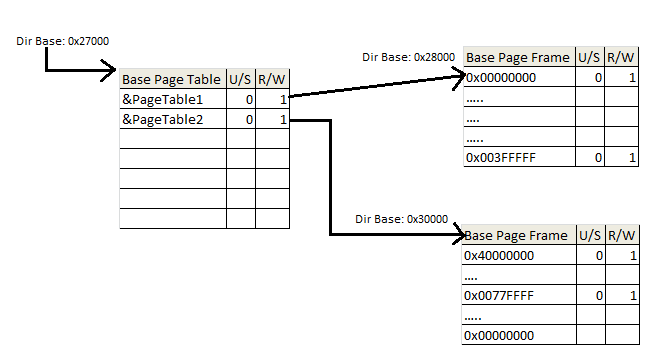
\includegraphics[scale=0.6]{imagenes/tablasDePaginasEj3.png}

\subsubsection{Activaci\'on de paginaci\'on}

Luego de armar el directorio de p\'aginas podemos habilitar la paginaci\'on. Para esto seguimo los siguientes pasos:
\begin{itemize}
 \item Cargar en CR3 la direccion al inicio del directorio de p\'aginas.
 \item Setear el bit mas significativo del registro CR0.
\end{itemize}


\newpage
\subsection{Ejercicio 4. Paginaci\'on de tareas}

\subsubsection{Paginaci\'on de las tareas}

Para la paginaci\'on de tareas se necesitaron los siguientes m\'odulos por cada tarea:
\begin{itemize}
 \item Inicializar un directorio de p\'aginas con 3 entradas, 2 para el Kernel iguales a las descriptas en el ejercicio 3 (es decir, identity mapping) 
 y una para direccionar a las p\'aginas de c\'odigo y pilas de cada tarea. Este Page directory est\'a definido en la direccion 0x40000000
 \item Dentro de la Page Table de las tareas se encuentran definidas las entradas de cada p\'agina de la tarea. Estas son, 2 entradas para
el c\'odigo de la tarea, 1 para el ancla y (cosa que no fue necesaria pero nos simplifico a la hora de codear) 1 para la pila nivel 0.
\end{itemize}

Con el fin de simplificar la cantidad de pasos, las direcciones fisicas de las paginas cada tarea estaran mapeadas en arrays externos. De esta forma no
tendremos que buscar dentro de la GDT para buscar una direccion fisica a la hora de hacer otras operaciones, que puede ser costoso en cuestiones de tiempo
y dejar un codigo poco claro.

A diferencia del ejercicio anterior, como en este caso estamos mapeando tareas, estas se diferencian de las p\'aginas de Kernel en que
los attributos que utilizan son diferentes, es decir, las tareas al correr en nivel 3 requieren que sus Page Directory entries y sus
Page table entries posean U/S = 1. De lo contrario no puedo acceder a esas p\'aginas como nos lo demostro\'o nustra experiencia en la
implementaci\'on.

El siguiente esquema explica mas simplemente lo nombrado anteriormente. Tener en cuenta que esto debe realizarse por cada tarea y que si
bien cada una est\'a mapeada al mismo lugar, la base del Page Directory es distinto para cada tarea, provocando que cada una tenga su
propio mapeo. Para empezar, page directory entry que corresponde a la tarea, es la 0x100 ya que 0x40000000 es una direccion virtual entonces
la tenemos que decodificar como 

\begin{center}
  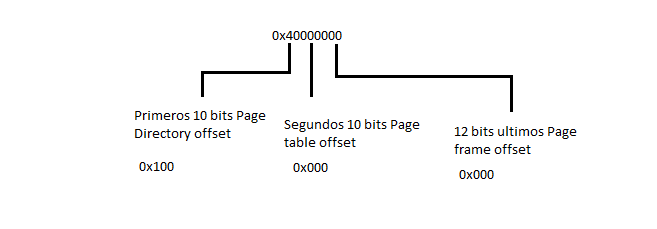
\includegraphics[scale=0.6]{imagenes/ComoDividoVirtual.png} 
\end{center}

Y Luego de esto el esquema de paginaci\'on nos quedar\'ia algo as\'i:

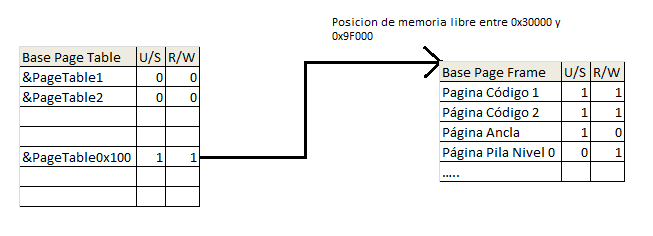
\includegraphics[scale=0.6]{imagenes/paginacionTareas.png}

Cabe destacar que para poder cumplir con los ejercicios siguientes, una tarea IDLE va a tener que ser mapeada al comienzo de la paginaci\'on
de lo contrario, no tener una tarea mapeada me imposibilita arrancar el sistema de scheduling que ser\'a introducido mas adelante.\footnote{Ver
secci\'on Ejercicio 7, Scheduling.}

\newpage
\subsection{Ejercicio 5 IDT / Clocks, Teclados, Syscalls y Banderas}

La siguiente secci\'on est\'a dedicada a los \emph{Handlers} o manejadores de las interrupciones. Estos son los c\'odigos que se ejecutan
cuando alguna porci\'on del systema produce un error o llama a una interrupci\'on mejor conocida como syscall o servicios del sistema.\\
Nuestro Kernel cuenta con 4 interrupciones que poseen handlers. Estas fueron mencionadas en el punto 3. Procederemos a explicar cada una de
ellas:
\begin{itemize}
 \item Clock: El clock es una interrupci\'on que se ejecuta cada ciertos ticks de reloj. La misma se encarga de buscar el siguiente selector
de segmento según es especificado en la secci\'on 7. y realizar el salto a dicho selector que puede corresponder a una tarea, una bandera o 
la tarea IDLE.
 \item Teclado: La interrupci\'on de teclado cumple la funci\'on de cambiar el estado de la pantalla entre el mapa si la ''m'' es presionada
y el estado de las banderas y las tareas corriendo si la ''e'' es presionada.
 \item Servicios o Syscalls: Esta interrupci\'on brinda al systema una serie de servicios o funciones a las tareas:
  \begin{itemize}
   \item Fondear: Se accede pasando por par\'ametro el n\'umero 0x923.Esta funci\'on permite a la tarea mover por tierra el ancla permitiendole 
mirar de a una p\'agina por vez en tierra. Esta llama a la funci\'on implementada en C anclar() ubicada en mmu.c.
   \item Cañonear: Se accede pasando por par\'ametro el n\'umero 0x83A, la direccion virtual donde voy a disparar y el buffer de 97 bytes
que funciona como misil. B\'asicamente este servicio nos permite escribir en cualquier lugar del mar un buffer de 97 bytes haciendo que
en caso de que en esa direcci\'on se encontrara una tarea enemiga, sus p\'aginas sean corrompidas. Esta llama a la funci\'on canionear()
implementada en mmu.c
   \item Navegar: bajo el n\'umero 0xAEF, recibe las nuevas direcciones de las primer y segunda p\'aginas de c\'odigo de la tarea. Generando
que mi tarea se pueda mover por el mar sin ser atrapada por una tarea enemiga. Esta syscall llama a navegar() implementada en C en mmu.c.
  \end{itemize}
En este caso hemos añadido un handler de error extra que verifica que no sean llamadas por una bandera haciendo nuestro c\'odigo mas seguro.

 \item Bandera: Esta interrupci\'on se encarga de imprimir la bandera y dar la impresi\'on de movimiento como si una bandera flameara. Cabe 
destacar que solo puede ser llamada por una bandera. Si llega a ser llamada por una tarea la misma debe ser desalojada. Esta llama a Bandera()
implementada en sched.c
\end{itemize}

Cabe destacar que las funciones implementadas en C para las syscalls, navegar, canionear y anclar, se encuentran allí dado que manejan p\'aginas
de memoria haciendo que ubicarlas en mmu.c sea lo m\'as conveniente para aprovechar todas las funciones y estructuras utilizadas. En el 
caso de Bandera() se encuentra en sched.c por un raz\'on similar.

\newpage
\subsection{Ejercicio 6. TSS}

Para que el procesador pueda despachar, ejecutar o suspender multiples tareas, es necesario salvar el estado de las mismas. La arquitectura provee mecanismos para esto. El segmento de estado (TSS, Task State Segment), es el que se encarga de almacenar la informaci\'on del estado de una tarea.\\

Una tarea est\'a identificada por el selector de segmento de su TSS. Y a su vez la TSS es un segmento, por lo tanto debe estar descripto en la GDT junto con los descriptores de segmento de c\'odigo y datos.\\

Tenemos 8 tareas y definimos un total de 18 TSS, uno para cada tarea, uno para cada bandera de tarea, uno para la tarea Idle, y otro lo dejamos en blanco para la tarea inicial donde se hace el primer salto.\\
Las entradas de tss idle y la que est\'a en blanco tienen privilegio de kernel, mientras que las dem\'as est\'an configuradas con privilegios de usuario.\\
\\
Las TSS se actualizan solas con cada JUMP Far, permiti\'endonos as\'i volver m\'as tarde a esa tarea y no perder la informaci\'on de la misma. Por esto mismo es necesario "incializar" una TSS para que cuando entremos por primera vez la informacion
sea valida. Al momento de inicializar estos segmentos, cada tarea y su flag tendran TSS virtualmente identicas, con la excepcion del eip y pequenios cambios con respecto a las posiciones de las pilas.\\

Como selectores de segmentos de GDT usamos los que definimos para las tareas (es decir, los de nivel 3), y seteamos el RPL en 0x03 para evitar un GPE. 

Una de las grandes ventajas de estar trabajando con direcciones virtuales es que no tenemos que saber la direccion fisica exacta de cada tarea para inicializarlas. 
Sabemos que todas las tareas comparten ciertas direcciones virtuales, asi que implemente seteamos el directorio de pagina (CR3) correspondiente a esa tarea y podemos usar direcciones identicas para todas las tareas.
Como mencionamos antes, las banderas recibiran datos parecidos, con excepcion de las pilas que estaran corridas. (El eip que reciban sera indiferente por lo que explicamos mas abajo)
La pila de nivel 0 seria un caso especial, pero como se acordan de la seccion de paginacion, la mapeamos en la direccion virtual 0x4000 3000 con el fin de evitar tener que buscarla ahora.

Las TSS de las flags son un caso particular por dos razones. La primera es que el eip no es un valor que sepamos de antemano, sino que depende de cada tarea. Al final de cada tarea hay un offset guardado, que sumandolo a 0x4000 0000 nos da la direccion virtual 
de la funcion flag. La segunda es que queremos que flag se comporte como una funcion tradicional, es decir, que corra siempre del principio hasta el final (o ser interrumpida). En pocas palabras, no nos interesa la posicion donde estuvo la ultima corrida, sino
que nos intereseria volver siempre al comienzo.
\\
Para resolver esto generamos dos funciones que definen el eip del TSS de un flag forma dinamica, y que deben ser corridas antes de saltar a un flag. Por un lado tenemos la funci\'on fetch\_eip, que se encarga de averiguar
el offset de la bandera buscando la tarea en la memoria (recordar que las tareas "navegan" y en teor\'ia podrian mutar), y la funci\'on reset\_eip, que escribe este dato dentro de la TSS.\\
\\

\newpage
\subsection{Ejercicio 7. Scheduller}

El Scheduller es la estructura mas grande y quizas mas compleja de nuestro trabajo. Su funcion es simple, coordinar en 
que orden ocurren los eventos en nuestro OS y determinar ciertas acciones como si una bandera excedio el tiempo que le es dado.\\
\\
Conceptualmente nos imaginamos al Scheduler dividido en dos etapas o dos corridas: una corrida de tareas que es interrumpida por una corrida de banderas.
Hay un timer llamado quantum que dictamina cuantos ciclos le queda a la corrida de tareas hasta que sea interrumpido por la corrida de banderas.
La corrida de banderas se ejecuta y una vez terminada vuelve a la corrida de tareas con el quantum reiniciado.
\\
Corrida tarea:
\\
Task 1 -> Task 2 -> Task  3 ->/corrida bandera/ -> Task 4 -> ...
\\
Corrida bandera:
\\
/venir de corrida tarea/ -> Flag 1 -> Flag 2 -> Flag 3 -> Flag 4 -> Flag 5 -> Flag 6 -> Flag 7 -> Flag 8 -> /volver a corrida tarea/
\\
Ademas, separamos los estados del scheduler (llamado contexto en nuestro codigo) en 5 instancias distintas, EN_IDLE, EN_IDLE_TAREA, EN_IDLE_BANDERA, 
EN_TAREA y EN_BANDERA. Para los fines del trabajo, los dos primeros estados son precindibles, (EN_IDLE solo se usa cuando empieza la maquina o nos quedamos,
quedamos sin tareas / EN_IDLE_TAREA tiene las mismas funciones de EN_TAREA) pero decidimos agregarlos para mantener la coherencia de la estructura. De esta 
manera, hay 3 estados cuyas propiedas nos importan resaltar.
\\
EN_TAREA: indica que se esta/estaba corriendo una tarea. Si vuelve al scheduler, se debera continuar con la corrida de tareas o inicializar la corrida de banderas 
dependiendo del quantum.

EN_IDLE_BANDERA: indica que se esta en un idle despues de haber hecho una bandera y usado la interrupcion 66. Al volver al scheduler esta bandera no debe borrarse,
simplemente debe continuarse con la corrida de banderas. (o de haber terminado, volver a la corrida de tareas)

EN_BANDERA: indica que se esta corriendo una bandera. Si vuelve al scheduler, quiere decir que la bandera no termino de ejecutarse (A.k.a no llamo a la int 66), por lo cual 
debe ser desalojada y luego se debe continuar con la corrida de bandera. (o de tareas de haber terminado)

\\
La interrupcion de clock se encarga de realizar todos los saltos y cambios de tareas, exceptuando el salto a idle (que puede ser hecho en cualquier momento). El scheduller
es la structura que le informa hacia donde ir, siguiendo . De esta forma, mantenemos el codigo facilmente segmentado.

Una excepcion interesante es el caso en el que no querramos saltar a ningun lado sino seguir en la tarea actual. Por ejemplo, si me queda una sola tarea y estoy en la corrida
de tareas aun con quantum me gustaria pertenecer en esa tarea. Para esto el scheduller devuelve el selector de segmento 0, el cual es reconocido por el clock como una
instruccion para volver a la tarea anterior (iret) y no realizar ningun salto. (tratar de saltar a una tarea en uso daria error)


\newpage
\subsection{Screen}

La estructura screen tambi\'en es una parte integral del trabajo porque no solo se ocupa de mostrarle
la informaci\'on al usuario, en ella tambi\'en se guardan ciertos datos y se interpreta cierta informaci\'on.
Por esto mismo nos pareci\'o importante agregarle una secci\'on.\\
\\
Como dice el enunciado, nosotros creamos dos buffers, uno para el screen de mapa y otro para el screen 
de estado. Adem\'as agregamos un tercer buffer que indica que banderas hay en una misma posici\'on del mapa. De esta forma, si antes hab\'ia muchas p\'aginas en una misma posici\'on, cuando cambio de posici\'on se vallan todas menos uno sabremos qu\'e bandera qued\'o y nos ahorraremos tiempo de proceso.\\
\\
Nuestra pantalla de estado est\'a separada en 4 gr\'aficos distintos, la bandera, la tabla de errores (que se encuentra a la derecha), la tabla de p\'aginas de tareas (que se encuentra en la parte inferior) y los banderines (columna inferior con numeros). Todas tienen su propias funciones, y la ventaja que tienen es que solo se imprimen mientras una tarea este ocurriendo o cuando hay un error. De esta forma, sabemos que si una impresi\'on est\'a corriendo es por que esa tarea todavia no fue despejada, por lo que no nos hace falta revisarlo todo el tiempo.\\
\\
Tabla errores es una estructura que imprime el estado de una tarea al momento de romperse, es decir los registros. Esto excluye a las instancias en donde una tarea es despejada pero no cay\'o en una interrupci\'on de intel, es decir "cuando pasa malos par\'ametros a la interrupci\'on de servicios", "cuando llama a int 50 desde una bandera", "cuando llama a int 66 desde una tarea" y "cuando una bandera no llama a la int 66". Es importante resaltar que a pesar que seguimos las instrucci\'on de la catedra y usamos el manual de Intel, eflags parec\'ia estar imprimiendo informaci\'on erronea o "sucia".\\
\\
Tabla de paginas de tareas nos muestra la direcci\'on f\'sica de las 3 p\'aginas principales de cada tarea (P\'agina de c\'odigo 1, P\'agina de c\'odigo 2, y a donde esta anclada). Tambi\'en acumular\'a los errores de cada tarea, sirvi\'endonos como gu\'ia para saber por qu\'e fue liberada cada estructura.\\
\\
Los banderines son una lista de numeros en el fondo que nos indica la tarea actual si estamos en una corrida de tareas, y la bandera actual si estamos en una corrida de banderas. Si una tarea ya fue despejada, esta aparecer\'a como una letra color gris para representar que no esta disponible.

\newpage
%%%%%%%%%%%%%%%%%%%%%%%%%%%%%%%%%%%%%%%%%%%%%%%%%%%%%%%%%%%%%%%%%%%%%%%%%%%%%%%
%% Conclusión                                                                %%
%%%%%%%%%%%%%%%%%%%%%%%%%%%%%%%%%%%%%%%%%%%%%%%%%%%%%%%%%%%%%%%%%%%%%%%%%%%%%%%



\end{document}